\section{Metodyka rozwiązania}
\label{sec:metodyka-rozwiazania}
W tej części opisane są szczegółowo metody rozwiązania postawionego problemu. Opis ten powinien być precyzyjny, wyczerpujący i zgodny z aktualnym formalizmem oraz terminologią specyficznymi dla dziedziny pracy. Powinien on w szczególności zawierać definicje stosowanych metod numerycznych, algorytmów oraz struktur danych.

\subsection{Rozwiązanie bazujące na standardzie telnet}
Finalnym produktem powinien być stabilny prototyp urządzenia, połączony z modułem ESP8266, posiadający przynajmniej jeden czujnik. Użytkownik powinien mieć możliwość zdalnego starowania tym urządzeniem za pomocą mobilnej aplikacji. System powinien składać się przynajmniej z trzech urządzeń, każde z nich powinno automatycznie łączyć się do sieci Wi-Fi po uruchomieniu. 

Dodatkowo, system powinien oferować wygodny interfejs dostępny dla użytkownika końcowego. Udostępnienie API poprzez sterowanie urządzeniami za pomocą telnetu pozwoli na programowy dostęp do sterowania urządzeń z poziomu dowolnego języka programowania. Powinny również zostać zaimplementowane mechanizmy autentykacji zlecanych operacji. Oprócz dostępu programowego, planowana jest implementacja graficznego interfejsu mobilnego, przeznaczonego dla użytkowników\cite{kukdm-art}.

\begin{figure}[!htbp]
	\centering
	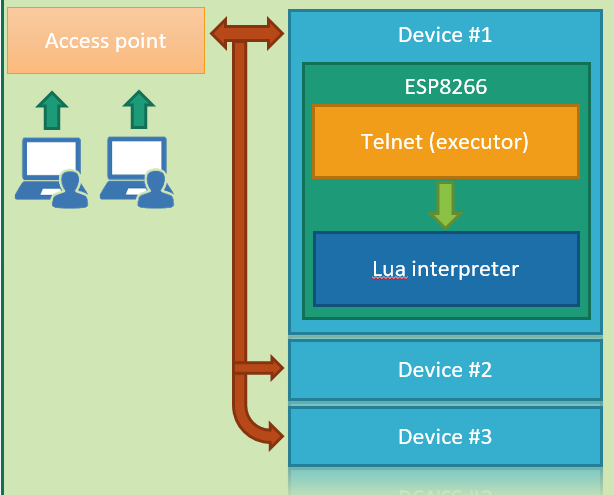
\includegraphics[width=0.9\textwidth]{images/fig01-arch-overview.png}
	\caption[Wizja architektury systemu.]{Wizja miejsca użytkownika, budowy urządzenia, oraz sposobu komunikacji}
	\label{fig:arch-overview}
\end{figure}

Wizję budowy urządzenia przedstawia \autoref{fig:arch-overview}.

\subsection{Rozwiązanie bazujące na CoAP Web Service}

\begin{figure}[!htbp]
	\centering
	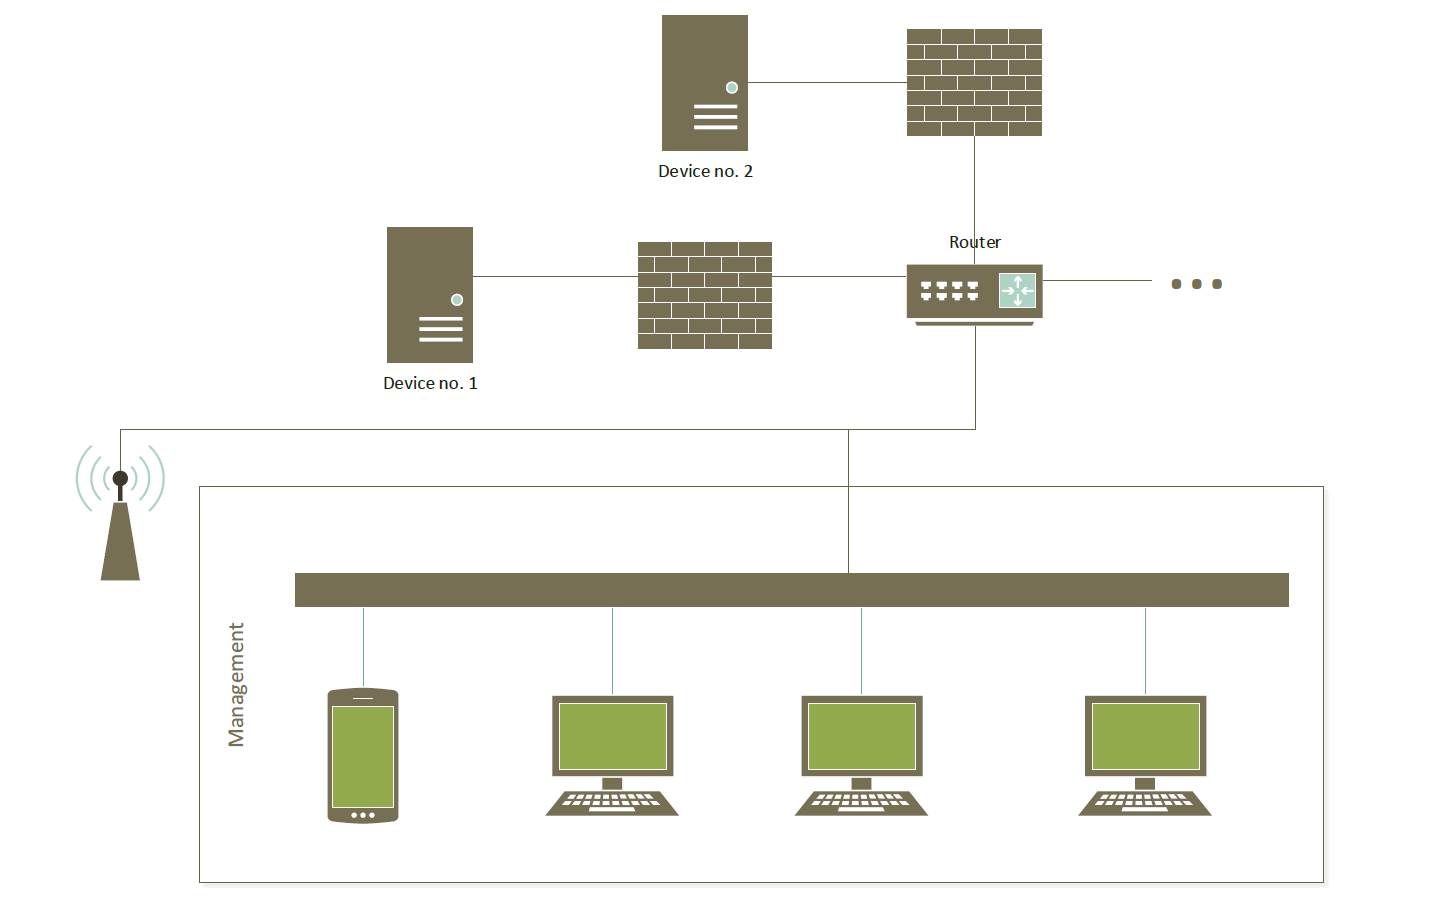
\includegraphics[width=0.9\textwidth]{images/schemat.png}
	\caption[Wizja architektury systemu w standardzie CoAP.]{Wizja miejsca użytkownika, sposobu komunikacji w systemie w standardzie CoAP}
	\label{fig:schemat}
\end{figure}
Wizję budowy urządzenia przedstawia \autoref{fig:schemat}.